\section{Complexity Analysis via Symbolic Execution Schemes}
\label{sec:symbolic}

\colorbox{yellow!20}{\textbf{TO INTRODUCTION}}
\begin{lstlisting}[basicstyle=\small]
   append$^o$ = fun a b ab ->
     ((a === Nil) /\ (ab === b)) \/
     (fresh (h t tb)
        (a === Cons(h, t)) /\
        (ab === Cons(h, tb) /\
        (append$^o$ t b tb)) 
     )
\end{lstlisting}

\colorbox{blue!20}{\parbox{\textwidth}{\textbf{PART 1}: Overview of the symbolic analysis approach.
Analyzing relational calls, symbolic variables as subset of logic variables, symbolic schemes, extracting approximations for d-measure and t-measure, solving approximations in metatheory.}}

For clarity we will provide demonstration of the complexity analysis for a specific example -- \lstinline|append$^o$| relation the introduction  -- throughout the section.

\colorbox{blue!20}{\parbox{\textwidth}{\textbf{PART 2}: Symbolic variables and symbolic analysis problem statement.}}

\colorbox{blue!20}{\parbox{\textwidth}{Substituting logic variables by ground values, valuations $\rho : V \to \grterms$}}

Extension for valuations:

\begin{definition}
  Suppose $V \subset U \subset \mathcal{A}$, $\rho \colon V \to \mathcal{T}_{\emptyset}$, and $\rho^\prime \colon U \to \mathcal{T}_{\emptyset}$. We say that $\rho^\prime$ extends $\rho$ (denotation: $ \rho^\prime \succ \rho$) if $ \forall x \in V \,:\, \rho^\prime\,(x) = \rho\,(x) $
\end{definition}

Let's say we want to analyze what happen if we substitute first two argument of \lstinline|append$^o$| with ground variables and left the last argument free.

\colorbox{blue!20}{\parbox{\textwidth}{Stability wrt free variables, counter and substitution}}

It is important to note that both our time measures are ``stable'' w.r.t. renaming of logical variables and change of counter of fresh logical variables (as long as it stays adequate).

\begin{replemma}{lem:measures_changing_env}

  Suppose

  \vskip-2mm\begin{gather*}
      FV\,(g) \cup \Dom\,(\sigma) \cup \VRan\,(\sigma) \subseteq \{ \alpha_1\dots\alpha_n \} \\
      FV\,(g^\prime) \cup \Dom\,(\sigma^\prime) \cup \VRan\,(\sigma^\prime) \subseteq \{ \alpha_1\dots \alpha_{n^\prime} \}
    \end{gather*}
  
  and there is a bijective substitution $\pi \colon FV\,(g \sigma) \to FV\,(g^\prime \sigma^\prime)$ such that $g \sigma \pi = g^\prime \sigma^\prime$. Then

  \vskip-3mm\begin{gather*}
    d\,(\taskst{g}{\mkenv{\sigma}{n}}) = d\,(\taskst{g^\prime}{\mkenv{\sigma^\prime}{n^\prime}})\\
    t\,(\taskst{g}{\mkenv{\sigma}{n}}) = t\,(\taskst{g}{\mkenv{\sigma}{n}})
  \end{gather*}

\end{replemma}

So the following definition will be useful to construct a base-state representative for an arbitrary goal.

\begin{definition} Let $g$ be a goal. An initial state for $g$ is

  \[
   init\,(g)=\taskst{g}{(\varepsilon, \ninit\,(g))}
  \]

  where
  
  \[ n_{init}\,(g) = \min\, \{ n \mid FV\,(g) \subseteq \{ \alpha_1\dots\alpha_n \} \} \]
\end{definition}

So we will be studying the family of queries \[ q^{app}(\mathbf{a}, \mathbf{b}) = init\,(\texttt{append$^o$} \, \mathbf{a} \, \mathbf{b} \, ab^?) \]

\colorbox{blue!20}{\parbox{\textwidth}{Symbolic unifications. Use usual unificatoion, but add constrains on symbolic variables}}

Notions for constrains:

\[
\upd{U}{\delta} = \begin{cases}
                           U & \quad\forall x \in U : FV\,(\delta\,(x)) \subset U \\
                           \upd{U \cup \displaystyle\bigcup\limits_{x \in U} FV\,(\delta\,(x))}{\delta} & \quad\mbox{otherwise}
                          \end{cases}
\]

\[ \constr{\delta}{U} = \{ x = \delta\,(x) \mid x \in U \cap \mathcal{D}om\,(\delta) \} \]

Soundness of symbolic unification:

\begin{replemma}{lem:symbolic_unification_soundness}

  Let $t_1$, $t_2$ be terms,  $V \subset \mathcal{A}$ and $\rho \colon V \to \grterms$. If $mgu\,(t_1, t_2) = \delta$ and
  $U = \upd{V}{\delta}$ then $t_1 \rho$ and $t_2 \rho$ are unifiable iff there is some $\rho' \colon U \to \grterms$ such that $\rho' \succ \rho$ and $\forall (y, \, t) \in \constr{\delta}{U}\,:\, \rho'\,(y) = t \rho'$. In such case $\rho'$ is unique and $ \rho \circ mgu\,(t_1 \rho, t_2 \rho) = \delta\circ\rho' $ up to alpha-equivalence (e.g. there exists a permutation $\pi$ on $FV(t_1) \cup FV(t_2)$, s.t. $ \rho \circ mgu\,(t_1 \rho, t_2 \rho) = \delta \circ\rho'\circ \pi$).
\end{replemma}


\colorbox{blue!20}{\parbox{\textwidth}{\textbf{PART 3}: Symbolic schemes. Form and derivation rules}}

We build schemes in the following form.

\[
\renewcommand{\arraystretch}{3}
\begin{array}{ccm{0.5cm}m{3cm}m{4cm}m{4cm}}
  \schemewithvset{\mathfrak{S}}{V} & = && \schemenode{$\unigoal{\mathcal{T}_\mathcal{A}}{\mathcal{T}_\mathcal{A}}$} & \schemenode{$\invokegoal{R^k}{\mathcal{T}_\mathcal{A}}{\mathcal{T}_\mathcal{A}}$} 
                                       & \multirow{2}{*}{\schemefork{$\schemewithvset{\mathfrak{S}}{V}$}{$\schemewithvset{\mathfrak{S}}{V}$}} \\
                                   &   && \schemesarrow{$\unigoal{\mathcal{T}_\mathcal{A}}{\mathcal{T}_\mathcal{A}}$}{$\{\mathcal{A}=\mathcal{T}_\mathcal{A}\}$}{$\schemewithvset{\mathfrak{S}}{U}$}
                                       & \schemedarrow{$\invokegoal{R^k}{\mathcal{T}_\mathcal{A}}{\mathcal{T}_\mathcal{A}}$}{$(\mathcal{T}_\mathcal{A}, \dots, \mathcal{T}_\mathcal{A}) \in \sembr{R^k}$}{$\schemewithvset{\mathfrak{S}}{U}$}
                                       & 
\end{array}
\]

The rules for building a scheme have the following form. \[ \schemetrans{g}{\Gamma}{\sigma}{n}{V}{\schemewithvset{\mathfrak{S}}{V}} \]

They are shown on \figureword~\ref{fig:scheme_formation}.

\begin{figure}[t]  
\renewcommand{\arraystretch}{2}
  \[
\begin{array}{cr}
  \onepremrule
		{  \schemetrans{g_1}{g_2 : \Gamma}{\sigma}{n}{V}{\schemewithvset{\mathfrak{S}}{V}}  } 
		{  \schemetrans{\conjgoal{g_1}{g_2}}{\Gamma}{\sigma}{n}{V}{ \schemewithvset{\mathfrak{S}}{V} }  } & \ruleno{Conj$_\mathfrak S$}
		\\
 \onepremrule
		{  \schemetrans{\substitute{g}{\alpha_n}{x}}{\Gamma}{\sigma}{n + 1}{V}{\schemewithvset{\mathfrak{S}}{V}}  }
		{  \schemetrans{\freshgoal{x}{g}}{\Gamma}{\sigma}{n}{V}{ \schemewithvset{\mathfrak{S}}{V} }  } & \ruleno{Fresh$_\mathfrak S$}\\
                
  % \multicolumn{3}{c}{
  \twopremrule
		{  \schemetrans{g_1}{\Gamma}{\sigma}{n}{V}{\schemewithvset{\mathfrak{S_1}}{V}}  }
		{  \schemetrans{g_2}{\Gamma}{\sigma}{n}{V}{\schemewithvset{\mathfrak{S_2}}{V}}  }
		{  \schemetrans{\disjgoal{g_1}{g_2}}{\Gamma}{\sigma}{n}{V}{\parbox[m]{2cm}{ \schemefork{$\schemewithvset{\mathfrak{S_1}}{V}$}{$\schemewithvset{\mathfrak{S_2}}{V}$}} }  } & \ruleno{Disj$_\mathfrak S$}\\ 
		

 %\multicolumn{3}{c}{
  \schemetrans{\unigoal{t_1}{t_2}}{\epsilon}{\sigma}{n}{V}{\parbox[m]{2cm}{\schemenode{$\unigoal{t_1 \sigma}{t_2 \sigma}$}}}& \ruleno{UnifyLeaf$_\mathfrak S$}\\

 %\multicolumn{3}{c}{
 \schemetrans{\invokegoal{R^k}{t_1}{t_k}}{\epsilon}{\sigma}{n}{V}{\parbox[m]{2cm}{\schemenode{$\invokegoal{R^k}{t_1 \sigma}{t_k \sigma}$}}}& \ruleno{InvokeLeaf$_\mathfrak S$}\\ 
		
 %\multicolumn{3}{c}{
  \onepremrule
		{  \nexists mgu\,(t_1 \sigma, t_2 \sigma)  }
		{  \schemetrans{\unigoal{t_1}{t_2}}{g : \Gamma}{\sigma}{n}{V}{\parbox[m]{2cm}{\schemenode{$\unigoal{t_1 \sigma}{t_2 \sigma}$}}} }& \ruleno{UnifyFail$_\mathfrak S$}\\

 %\multicolumn{3}{c}{
  \threepremrule
		{  mgu\,(t_1 \sigma, t_2 \sigma) = \delta  }
		{  U = \upd{V}{\delta}  }
		{  \schemetrans{g}{\Gamma}{\sigma \delta}{n}{U}{\schemewithvset{\mathfrak{S}}{U}}  }
		{  \schemetrans{\unigoal{t_1}{t_2}}{g : \Gamma}{\sigma}{n}{V}{\parbox[m]{2cm}{\schemesarrow{$\unigoal{t_1 \sigma}{t_2 \sigma}$}{$\constr{\delta}{U}$}{$\schemewithvset{\mathfrak{S}}{U}$}} }   } & \ruleno{UnifySuccess$_\mathfrak S$}\\
		
 %\multicolumn{3}{c}{
  \twopremrule
		{  \mbox{\phantom{XXXXXX}} U =  V \cup \displaystyle\bigcup\limits_{i} FV\,(t_i \sigma) }
		{  \schemetrans{g}{\Gamma}{\sigma}{n}{U}{\schemewithvset{\mathfrak{S}}{U}} \mbox{\phantom{XXXXXX}} }
		{  \schemetrans{\invokegoal{R^k}{t_1}{t_k}}{g : \Gamma}{\sigma}{n}{V}{ \parbox[m]{2cm}{\schemedarrow{$\invokegoal{R^k}{t_1 \sigma}{t_k \sigma}$}{$ (t_1 \sigma, \dots, t_k \sigma) \in \sembr{R^k} $}{$\schemewithvset{\mathfrak{S}}{U}$}} }   } & \ruleno{Invoke$_\mathfrak S$}
 \end{array}
\]
\caption{Scheme Formation Rules}
\label{fig:scheme_formation}
\end{figure}

The scheme for our example is shown in \figureword~\ref{fig:example_scheme}.

\begin{figure}[t]
\begin{center}
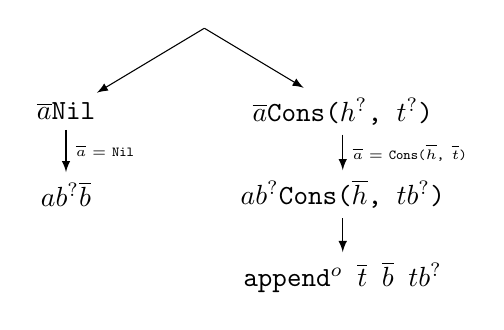
\begin{tikzpicture}[level distance=30pt, sibling distance=10em, edge from parent/.style={draw,-latex}]
   \coordinate   
      child { node {$\unigoal{\overline{a}}{\texttt{Nil}}$}
        child { node {$\unigoal{ab^?}{\overline{b}}$}
                  edge from parent node[right]{\tiny{$\overline{a} = \texttt{Nil}$}} } }
      child { node {$\unigoal{\overline{a}}{\texttt{Cons($h^?$, $t^?$)}}$} 
      	child { node {$\unigoal{ab^?}{\texttt{Cons($\overline{h}$, $tb^?$)}}$}
      	   child { node {\texttt{append$^o$ $\overline{t}$ $\overline{b}$ $tb^?$}} }
      	   edge from parent node[right]{\tiny{$\overline{a} = \texttt{Cons($\overline{h}$, $\overline{t}$)}$}}  } } ;
\end{tikzpicture}
\end{center}

\caption{Symbolic execution scheme for the goal $\texttt{append$^o$} \, a^? \, b^? \, ab^?$ with initial $V = \{ a^?, b^? \}$. Variables from the set of ground variables $V$ for each node are overlined (on edges variables are overlined in accordance with $V$ for the next node). }
\label{fig:example_scheme}
\end{figure}

%\FloatBarrier

\colorbox{blue!20}{\parbox{\textwidth}{\textbf{PART 4}: Extracting recursive approximations.}}

Here are the traversals of scheme that will be used for approximations. For a scheme $\schemewithvset{\mathfrak{S}}{V}$ it is a function from a valuation $\rho \colon V \to \grterms$ to natural numbers (for $\mathcal{D}$ and $\mathcal{T}$) or to sets of base-states (for $\mathcal{L}$).

\begin{figure}[t]
\[
\begin{array}{rclcl}
 \mathcal{\nicefrac{D}{T}}\,(&\parbox[m]{1.3cm}{\schemenode{$\unigoal{t_2}{t_2}$}}&)(\rho) &=& 1  \\

 \mathcal{\nicefrac{D}{T}}\,(&\parbox[m]{2.5cm}{\schemenode{$\invokegoal{R^k}{t_1}{t_k}$}}&)(\rho) &=& \nicefrac{d}{t}\,(\taskst{\invokegoal{R^k}{t_1 \rho}{t_k \rho}}{e_{init}}) \\

 \mathcal{\nicefrac{D}{T}}\,(&\parbox[m]{2cm}{\schemesarrow{$\unigoal{t_1}{t_2}$}{$Cs$}{$\schemewithvset{\mathfrak{S}}{U}$}} &)(\rho) &=& 1 +
      \sum\limits_{\substack{ \rho' \colon V \to \grterms \\
                                      \rho' \succ \rho \\
                                      \forall (y, t) \in Cs\,:\, \rho'\,(y) = t\, \rho'  }}
           \mathcal{\nicefrac{D}{T}}\,(\schemewithvset{\mathfrak{S}}{U})(\rho')  \\

 \mathcal{\nicefrac{D}{T}}\,(& \parbox[m]{4cm}{\schemedarrow{$\invokegoal{R^k}{t_1}{t_k}$}{ $(t_1, \dots, t_k) \in \sembr{R^k}  $}{$\schemewithvset{\mathfrak{S}}{U}$}} &)(\rho) &=&
      \nicefrac{d}{t}\,(\taskst{\invokegoal{R^k}{t_1 \rho}{t_k \rho}}{e_{init}}) +
      \sum\limits_{\substack{ \rho' \colon V \to \grterms \\
                                      \rho' \succ \rho \\
                                      (t_1 \rho', \dots, t_k \rho') \in \sembr{R^k}  }}
           \mathcal{\nicefrac{D}{T}}\,(\schemewithvset{\mathfrak{S}}{U})(\rho')  \\

 \mathcal{\nicefrac{D}{T}}\,(&\parbox[m]{2.5cm}{\schemefork{$\schemewithvset{\mathfrak{S}_1}{V}$}{$\schemewithvset{\mathfrak{S}_2}{V}$}}&)(\rho) &=&
 \mathcal{\nicefrac{D}{T}}\,(\schemewithvset{\mathfrak{S}_1}{V})(\rho) + \mathcal{\nicefrac{D}{T}}\,(\schemewithvset{\mathfrak{S}_2}{V})(\rho)
\end{array}
\]
\caption{Complexity Measures Extraction: $\mathcal D$ and $\mathcal T$}
\label{fig:scheduling_extraction_d_t}
\end{figure}


\begin{figure}[t]
\[
\begin{array}{rclcl}
 \mathcal{L}\,(&\parbox[m]{1.3cm}{\schemenode{$\unigoal{t_2}{t_2}$}}&)(\rho) &=& \{\taskst{\unigoal{t_2}{t_2}}{e_{init}}\} \\

 \mathcal{L}\,(&\parbox[m]{2.5cm}{\schemenode{$\invokegoal{R^k}{t_1}{t_k}$}}&)(\rho) &=& \{\taskst{\invokegoal{R^k}{t_1 \rho}{t_k \rho}}{e_{init}}\} \\

 \mathcal{L}\,(&\parbox[m]{2cm}{\schemesarrow{$\unigoal{t_1}{t_2}$}{$Cs$}{$\schemewithvset{\mathfrak{S}}{U}$}} &)(\rho) &=&  \{\taskst{\unigoal{t_2}{t_2}}{e_{init}}\} \cup
      \bigcup\limits_{\substack{ \rho' \colon V \to \grterms \\
                                      \rho' \succ \rho \\
                                      \forall (y, t) \in Cs\,:\, \rho'\,(y) = t\, \rho'  }}
           \mathcal{L}\,(\schemewithvset{\mathfrak{S}}{U})(\rho')  \\

 \mathcal{L}\,(& \parbox[m]{4cm}{\schemedarrow{$\invokegoal{R^k}{t_1}{t_k}$}{ $(t_1, \dots, t_k) \in \sembr{R^k}  $}{$\schemewithvset{\mathfrak{S}}{U}$}} &)(\rho) &=&
      \{\taskst{\invokegoal{R^k}{t_1 \rho}{t_k \rho}}{e_{init}}\} \cup
      \bigcup\limits_{\substack{ \rho' \colon V \to \grterms \\
                                      \rho' \succ \rho \\
                                      (t_1 \rho', \dots, t_k \rho') \in \sembr{R^k}  }}
           \mathcal{L}\,(\schemewithvset{\mathfrak{S}}{U})(\rho')  \\

 \mathcal{L}\,(&\parbox[m]{2.5cm}{\schemefork{$\schemewithvset{\mathfrak{S}_1}{V}$}{$\schemewithvset{\mathfrak{S}_2}{V}$}}&)(\rho) &=&
 \mathcal{L}\,(\schemewithvset{\mathfrak{S}_1}{V})(\rho) \cup \mathcal{L}\,(\schemewithvset{\mathfrak{S}_2}{V})(\rho)
\end{array}
\]
\caption{Complexity Measures Extraction: $\mathcal L$}
\label{fig:scheduling_extraction_l}
\end{figure}

\colorbox{yellow!20}{\parbox{\textwidth}{Maybe desribe DNF and call requirements informally?}}

We prove the theorem only for goals in DNF.

\[
\begin{array}{lcl}
B_{nf} & = &  \unigoal{\mathcal{T}_\mathcal{X}}{\mathcal{T}_\mathcal{X}} \; \mid \;
                     \invokegoal{R^k}{\mathcal{T}_\mathcal{X}}{\mathcal{T}_\mathcal{X}} \\
C_{nf} & = & B_{nf} \; \mid \; \conjgoal{C_{nf}}{B_{nf}} \\
F_{nf} & = & C_{nf} \; \mid \; \freshgoal{X}{F_{nf} } \\
D_{nf} & = & F_{nf} \; \mid \; \disjgoal{D_{nf}}{F_{nf}}
\end{array}
\]

We also have a requirement that all recursive calls performed during unification are \emph{grounding} and \emph{non-repetitive}.

\begin{definition}
  We call relational invocation
  
  \[\taskst{\invokegoal{R^k}{t_1}{t_k}}{e}\]

  \emph{grounding} and \emph{non-repetitive} if 

  \vskip-2mm\begin{gather*}
    \forall (\sigma^{a}, n^{a}) \in \tra{\taskst{\invokegoal{R^k}{t_1}{t_k}}{e}} \,:\, FV(t_i \sigma^{a}) = \emptyset\\
    \forall (\sigma_1^{a},\, n_1^{a}),\, (\sigma_2^{a},\, n_2^{a}) \in \tra{\taskst{\invokegoal{R^k}{t_1}{t_k}}{e}} \,:\, (t_1 \sigma_1^{a}, \dots, t_k \sigma_1^{a}) \ne (t_1 \sigma_2^{a},\, \dots, t_k \sigma_2^{a})
  \end{gather*}
\end{definition}

The following main theorem provides the principal recursive approximations, extracted from the scheme for a given goal.

\begin{reptheorem}{extracted_approximations}
Let $g \in D_{nf}$ and all sub-calls encountered during its evaluation are grounding and non-repetitive, and let

\[  \schemetrans{g}{\epsilon}{\varepsilon}{n_{init}(g)}{V}{\schemewithvset{\mathfrak{S}}{V}}  \]

\noindent Then

\[
\begin{array}{rcl}
    d\,(init\,(g\,\rho)) &=& \mathcal{D}\,(\schemewithvset{\mathfrak{S}}{V})(\rho) + \Theta\,(1) \\
   t\,(init\,(g\,\rho)) &=& \mathcal{T}\,(\schemewithvset{\mathfrak{S}}{V})(\rho) + \Theta\,(\mathcal{D}\,(\schemewithvset{\mathfrak{S}}{V})(\rho)
   - \maxd\limits_{\taskst{g_i}{e_i} \in \mathcal{L}(\schemewithvset{\mathfrak{S}}{V})(\rho)} d\,(\taskst{g_i}{e_i}) + 1)
\end{array}
   \]
  being considered as functions on

  \[\rho \colon V \to T_{\emptyset}\]
\end{reptheorem}

It is based on the  \lemmaword~\ref{lem:symbolic_unification_soundness}, \lemmaword~\ref{lem:sum_estimation}, generalization of the \lemmaword~\ref{lem:times_measure_equations} and soundness and completeness of operational semantics w.r.t. the denotational one.

The traversing extracts the following recursive approximations for both measures from the scheme. Instead of passing mapping $\rho$ through the approximation, we will write it down as a dependency on ground values $\mathbf{a}$ and $\mathbf{b}$ that are values of $\rho$ on $a$ and $b$ respecively. We use values instead of valuations for nodes too.

\[
\begin{array}{lcll}
d(q^{app}(\mathbf{a}, \mathbf{b})) & = & & (1 + \sum\limits_{\overline{a} = \texttt{Nil}} 1) + (1 + \sum\limits_{\mathbf{h}, \mathbf{t}: \mathbf{a} = \texttt{Cons($\mathbf{h}$, $\mathbf{t}$)}} (1 + d(q^{app}(\mathbf{t}, \mathbf{b})))) \\
& & + \Theta( & 1) \\
\\
t(q^{app}(\mathbf{a}, \mathbf{b})) & = & & (1 + \sum\limits_{\overline{a} = \texttt{Nil}} 1) + (1 + \sum\limits_{\mathbf{h}, \mathbf{t}: \mathbf{a} = \texttt{Cons($\mathbf{h}$, $\mathbf{t}$)}} (1 + t(q^{app}(\mathbf{t}, \mathbf{b})))) + \\
& & + \Theta( & (1 + \sum\limits_{\overline{a} = \texttt{Nil}} 1) + (1 + \sum\limits_{\mathbf{h}, \mathbf{t}: \mathbf{a} = \texttt{Cons($\mathbf{h}$, $\mathbf{t}$)}} (1 + d(q^{app}(\mathbf{t}, \mathbf{b})))) - \\
& & &  - \maxd\limits_{\mathbf{h}, \mathbf{t}: \mathbf{a} = \texttt{Cons($\mathbf{h}$, $\mathbf{t}$)}} d(q^{app}(\mathbf{t}, \mathbf{b})) + 1) 
\end{array}
\]


\colorbox{blue!20}{\parbox{\textwidth}{\textbf{PART 5:} simplification in matatheory.}}

Now we move into the metatheory to solve this systems of recursive approximations and deduce the complexity. As usual, when we add the informations from the metatheory the approximations became quite simple.

We consider two cases: when the first list is empty or not. Also, since there is only one non-trivial leaf in the scheme with only one enviroment, so we know that the excluded maximum is reached at the recursive call. After we exclude the recursive call from costs part, we get the following linear approximations. 

\[
\begin{array}{lcl}
d(q^{app}(\texttt{Nil}, \mathbf{b})) & = & \Theta(1) \\
d(q^{app}(\texttt{Cons($\mathbf{h}$, $\mathbf{t}$)}, \mathbf{b})) & = & d(q^{app}(\mathbf{t}, \mathbf{b})) + \Theta(1) \\
\\
t(q^{app}(\texttt{Nil}, \mathbf{b})) & = & \Theta(1) \\
t(q^{app}(\texttt{Cons($\mathbf{h}$, $\mathbf{t}$)}, \mathbf{b})) & = & t(q^{app}(\mathbf{t}, \mathbf{b})) + \Theta(1) \\
\end{array}
 \]
 
In this case the interleaving does not add a significant penalty, because we have recursive call in the end and its cost is eliminated. From these approximation it is clear that the complexity of both measures is linear on the length of the first argument.

\[
\begin{array}{lcl}
d(q^{app}(\mathbf{a}, \mathbf{b})) & = & \Theta(len(\mathbf{a})) \\
t(q^{app}(\mathbf{a}, \mathbf{b})) & = & \Theta(len(\mathbf{a})) \\
\end{array}
 \]
 
In contrast, for the naive version the $d$ would not be eliminated and we would have approximations

\[
\begin{array}{lcl}
d(q^{app}(\texttt{Nil}, \mathbf{b})) & = & \Theta(1) \\
d(q^{app}(\texttt{Cons($\mathbf{h}$, $\mathbf{t}$)}, \mathbf{b})) & = & d(q^{app}(\mathbf{t}, \mathbf{b})) + \Theta(1) \\
\\
t(q^{app}(\texttt{Nil}, \mathbf{b})) & = & \Theta(1) \\
t(q^{app}(\texttt{Cons($\mathbf{h}$, $\mathbf{t}$)}, \mathbf{b})) & = & t(q^{app}(\mathbf{t}, \mathbf{b})) + \Theta(d(q^{app}(\mathbf{t}, \mathbf{b})) ) \\
\end{array}
 \]

Which gives quadratic complexity.
